\documentclass{beamer}

% Theme and Color Setup
\usetheme{default}
\usecolortheme{seagull}

% Custom Color Definitions (OSU Branding)
\definecolor{osuorange}{RGB}{215, 63, 9}  % OSU Orange
\definecolor{osublack}{RGB}{0, 0, 0}      % Black
\definecolor{osugray}{RGB}{75, 75, 77}    % Dark Gray

% Use OSU colors for the title page, frame titles, and text
\setbeamercolor{title}{fg=osuorange}
\setbeamercolor{frametitle}{bg=osuorange, fg=white}
\setbeamercolor{structure}{fg=osuorange}
\setbeamercolor{normal text}{fg=osublack, bg=white}

% Title Page Information
\title[PTA Sensitivity]{Quick Sensitivity Curves for Pulsar Timing Arrays}
\subtitle{Making unrealistic sensitivity curves more realistic}
\author[Jeremy Baier]{Jeremy Baier}
\institute[OSU]{Oregon State University}
\date{\today}

\begin{document}

% Title Slide
\begin{frame}
    \titlepage
\end{frame}

% Outline Slide
\begin{frame}{Outline}
    \tableofcontents
\end{frame}

% SECTION 1: INTRODUCTION
\section{Introduction to Pulsar Timing Arrays}
\begin{frame}{Pulsars}
    \begin{itemize}
        \item Pulsars are rapidly rotating neutron stars that emit beams of radiation.
        \item "millisecond" pulsars are highly stable
        \item Can track changes in relative motion between Earth and pulsars
    \end{itemize}
    \begin{figure}
        \centering
        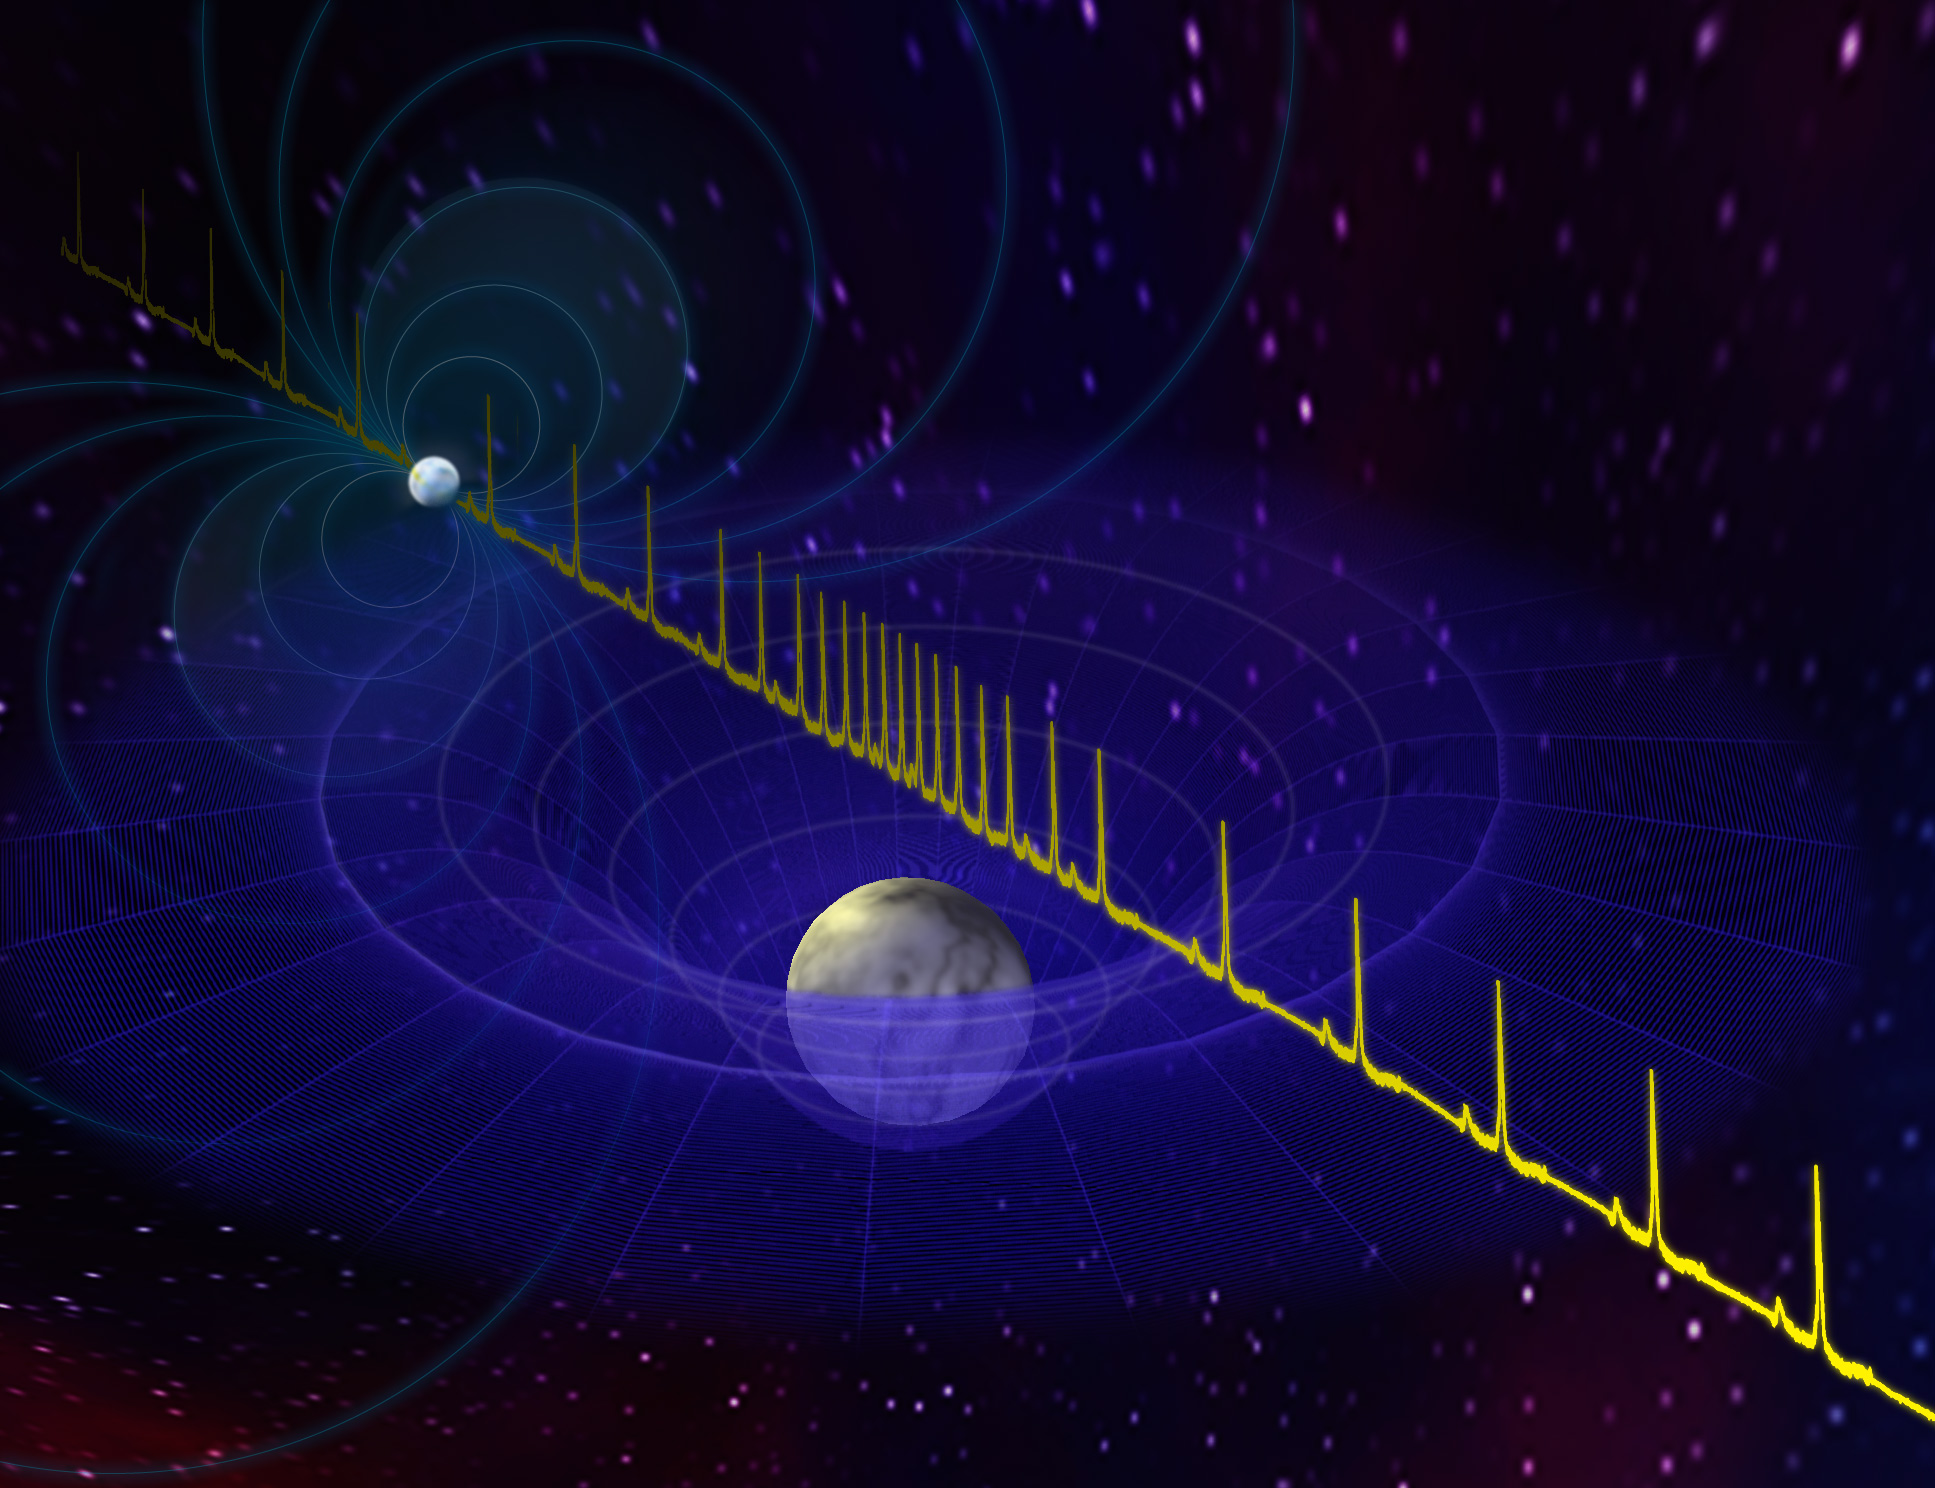
\includegraphics[width=0.5\linewidth]{figs/pulsar_timing.png}
        \caption{Relative motion of the earth and pulsar can be seen in the arrival times of pulses.}
        \label{fig:pulsar}
    \end{figure}
\end{frame}

\begin{frame}{Pulsars Timing Arrays (PTAs)}
\begin{itemize}
        \item an array of millisecond pulsars
        \item track relative changes in Earth-pulsar distance over decades
        \item correlations between pulsars across the sky reveal gravitational waves
    \end{itemize}
    \begin{figure}
        \centering
        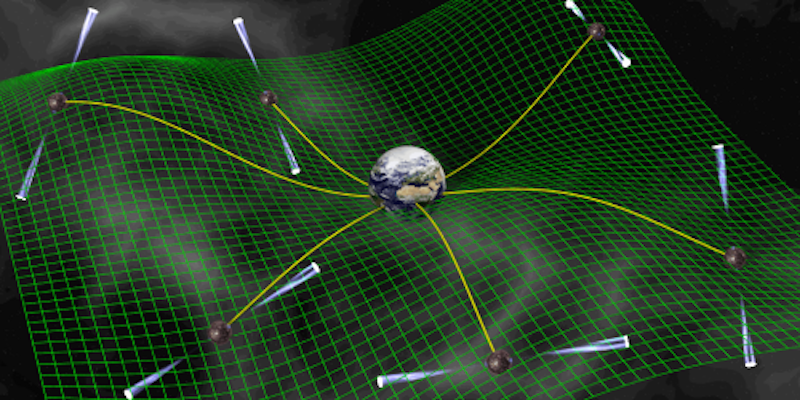
\includegraphics[width=0.75\linewidth]{figs/champion_pta.png}
        \caption{Artist rendering of a PTA}
        \label{fig:pulsar}
    \end{figure}
\end{frame}


\section{Sensitivity Curves}
\begin{frame}{Sensitivity Curves}
    In general, sensitivity curves are a way to characterize the sensitivity of a detector to a given signal.
    \begin{itemize}
        \item Encode the noise properties of the detector.
        \item Can be used to assess to the "detectability" of something.
        \item Useful figures of merit for detector characterization.
        \item tools exist to calculate the sensitivity curve for gravitational wave detectors ...
    \end{itemize}
\end{frame}

\begin{frame}{Sensitivity Curves}
    \begin{figure}
        \centering
        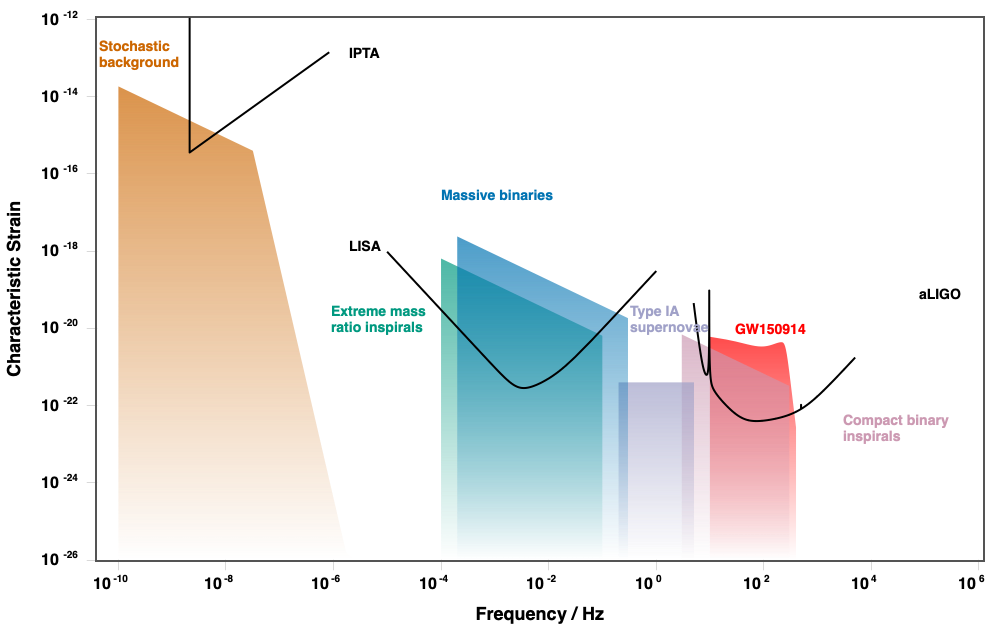
\includegraphics[width=\linewidth]{figs/gwplotter.png}
        \caption{Community resource for approximate GW sensitivity curves
        \centering \url{https://gwplotter.com/}
        }
        \label{fig:sensitivity_curve}
    \end{figure}
\end{frame}

\begin{frame}{Sensitivity Curves}
    But PTA sensitivity curves are not pizza slices !!
    \begin{figure}
        \centering
        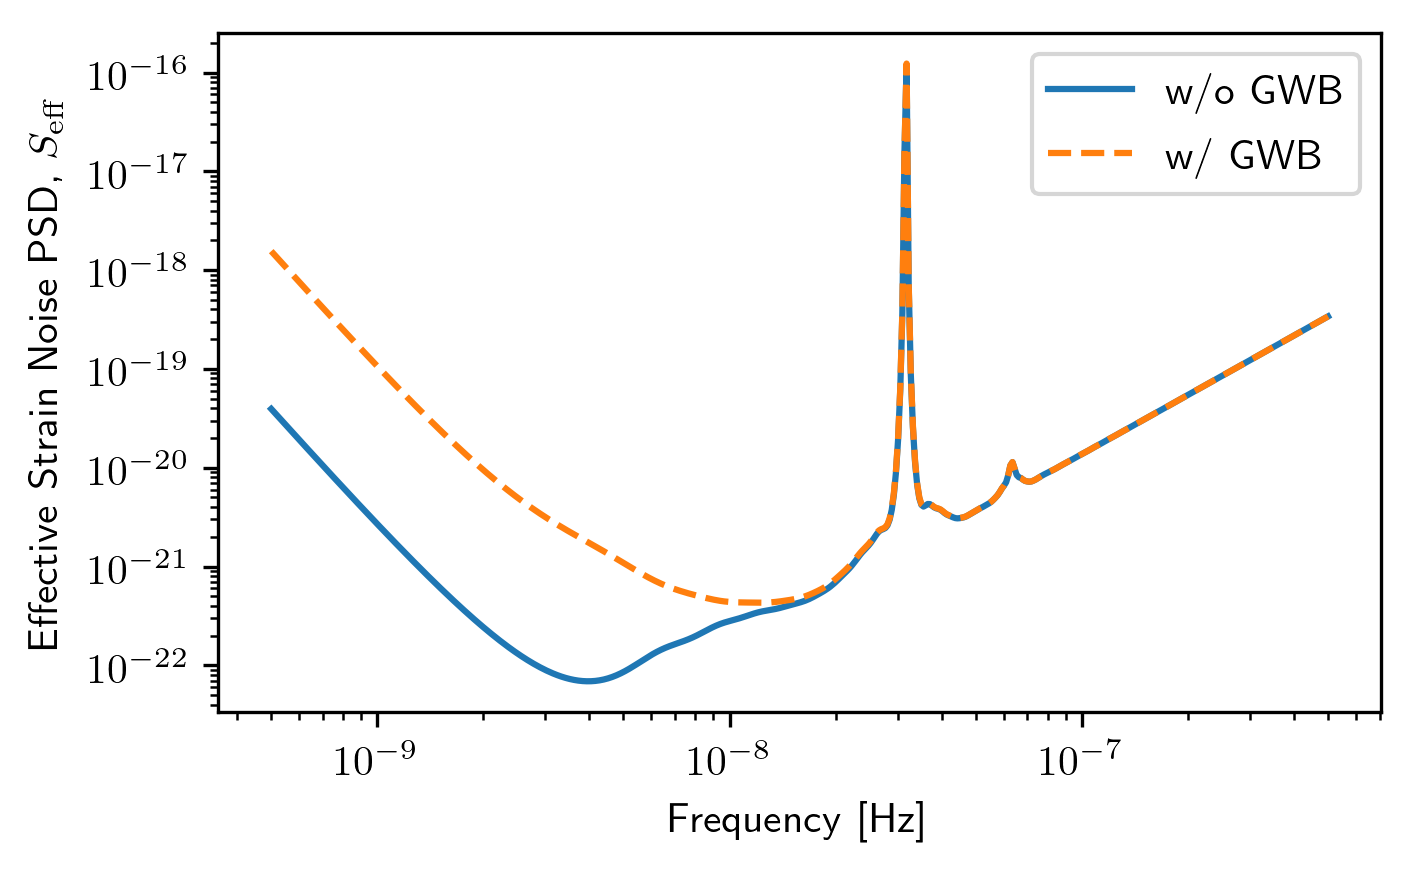
\includegraphics[width=\linewidth]{figs/example_sensitivity_curve.png}
        \caption{Example "realistic" sensitivity curve for a PTA
        \centering \url{https://hasasia.readthedocs.io}
        }
        \label{fig:pta_sensitivity_curve}
    \end{figure}
\end{frame}

\begin{frame}{Sensitivity Curves}
    Project goals:
    \begin{itemize}
        \item \textbf{derive a quick sensitivity curve for PTAs}
        \item implement quick sensitivity curve into \textit{GW Plotter}
        \item share with the rest of the GW astronomy community
    \end{itemize}
\end{frame}

\section{Derivation of Quick Sensitivity Curves}

\begin{frame}{Quick Sensitivity Curve Derivation}
    We will start from the realistic sensitivity curves presented in eq. 92 of Hazboun et al. (2019),
    \[
    S_{\text{eff}}(f) = \left( \sum_I \sum_{J > I} \frac{T_{IJ}}{T_{\text{obs}}} \frac{\chi_{IJ}^2}{S_I(f) S_J(f)} \right)^{-1/2}
    \]
    \begin{itemize}
        \item $S_{\text{eff}}$ is the effective background sensitivity
        \item $T_{\text{obs}}$: Total observational time span
        \item $T_{IJ}$: Overlapping observational time span between pulsars $I$ and $J$
        \item $\chi_{IJ}$: correlation coefficients
        \item $S_I(f)$: Individual pulsar sensitivity $I$
    \end{itemize}
\end{frame}

\begin{frame}{Derivation of Quick Sensitivity Curves}
    Simplifying assumptions from GW Plotter:
    \begin{itemize}
        \item Uniform distribution of pulsars across the sky
        \item Identical noise properties for all pulsars
        \item $T_I = T_{\rm obs}$ (all pulsars observed for full timespan)
        \item Same observational cadence for all pulsars
    \end{itemize}
\end{frame}

% Slide 5: Simplified Sensitivity Equation
\begin{frame}{Simplified Sensitivity Equation}
    Assuming uniform pulsar distribution across the sky,
    \[
    \chi_{IJ}^2 \approx 1/48
    \]
    \[
    S_{\text{eff}}(f) = \left( \sum_I \sum_{J > I} \frac{T_{IJ}}{T_{\text{obs}}} \frac{1}{48 \space S_I(f) S_J(f)} \right)^{-1/2}
    \]
    \pause
    Assuming that all pulsars have been observed for the total timespan, $T_{\rm obs}=T_{IJ}$,
    \[
    S_{\text{eff}}(f) = \left( \sum_I \sum_{J > I}\frac{1}{48 \space S_I(f) S_J(f)}\right)^{-1/2}
    \]
\end{frame}

\begin{frame}{Simplified Sensitivity Equation}
    Assuming that all pulsars have the same noise properties, $S_I\approx S_J$.
    So the sum can be simplified\ldots
    \[
    \sum_I \sum_{J > I} \frac{1}{48 \space S_I(f) S_J(f)} \approx \frac{N_{\rm psr}(N_{\rm psr}-1)}{2} \frac{1}{48 \space S_I(f)^2}
    \]
    And our expression for sensitivity becomes\ldots
    \[
    S_{\text{eff}}(f) = \left( \frac{N_{\rm psr}(N_{\rm psr}-1)}{2}\frac{1}{48 \space S_I(f)^2} \right)^{-1/2}
    \]

    So we only need to calculate the sensitivity for one pulsar!

\end{frame}


\begin{frame}{Final Sensitivity Equation}
    Single pulsar sensitivity is given by:
    \[
        S_{I}(f) = \frac{1}{\mathcal{N}_I^{-1}(f)\mathcal{R}(f)} = \frac{12\pi^2f^2}{\mathcal{N}_I^{-1}(f)}
        \]
        where $\mathcal{N}_I^{-1}(f)$ is the noise-weighted inverse transmission function for pulsar $I$.
    \pause
    \newline
    From the above equation, it follows that:
    \[
    S_{\text{eff}}(f) = \left(\frac{96}{N_{\rm psr}(N_{\rm psr}-1)}\right)^{1/2} \frac{12\pi^2f^2}{\mathcal{N}^{-1}_I(f)}
    \]
\end{frame}

\begin{frame}{Invserse Noise-Weighted Transmission}
    \[
    \mathcal{N}^{-1}(f) \equiv \frac{1}{2 T_{\text{span}}} \sum_{I,J} \left[ G \left( G^T C G \right)^{-1} G^T \right]_{I,J} e^{i 2 \pi f \left(t_i - t_j\right)},
    \]
    Most expensive part of the computation because C is an $N_{\rm toa} \times N_{\rm toa}$ covariance matrix.
    (memory intensive)
    \pause
    \newline

    So we approximate...
    \[
    \mathcal{N}^{-1}_I(f) \approx \frac{\mathcal{T}_I(f)}{P_{\rm N}(f)}
    \]
    where $\mathcal{T}_I(f) \approx \left(1 + \frac{1}{T_{\rm obs}f}\right)^{-6}$ is an approximation to the transmission function and $P_{\rm N}(f)$ is the power in the noise.
\end{frame}

\begin{frame}{Transmission Function}
    Here we use a first order polynomial approximation to the transmission function:
    \[
    \mathcal{T}_I(f) \approx \left(1 + \frac{1}{T_{\rm obs}f}\right)^{-6}
    \]
    The transmission function describes how much power we lose at each frequency due to our fit to a timing model.
    \begin{figure}
        \centering
        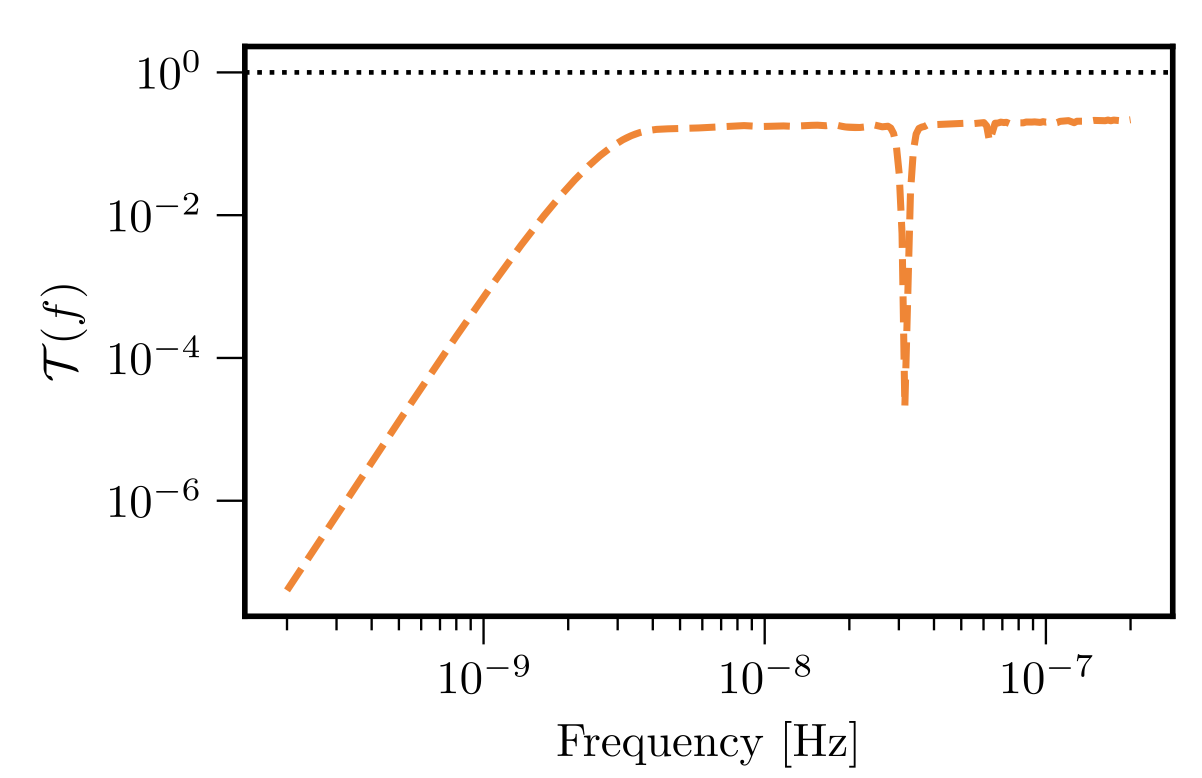
\includegraphics[width=0.5\linewidth]{figs/transmission_function.png}
        \caption{Example of an unapproximated transmission function.}
        \label{fig:transmission_function}
    \end{figure}
\end{frame}


\begin{frame}{Noise Power}
    The power in the noise is given by:
    \[
    P_{N} = P_{\rm WN} + P_{\rm RN} = 2\Delta t\sigma^2 + A_{\rm RN}f^{-\gamma_{\rm RN}}
    \]
    where 
    \begin{itemize}
        \item $\sigma$ is the time of arrival uncertainty
        \item $\Delta t$ is the observational cadence
        \item $A_{\rm RN}$ is the red-noise amplitude
        \item and $\gamma_{\rm RN}$ is the red-noise spectral index
    \end{itemize}
\end{frame}

\begin{frame}{Final Expression}

    Putting it all together, we have the final expression for the simplified sensitivity curve...
    \[
    S_{\text{eff}}(f) = \left(\frac{96}{N_{\rm psr}(N_{\rm psr}-1)}\right)^{1/2} \frac{12\pi^2f^2}{\mathcal{T}_I(f)P_{\rm N}(f)}
    \]
    \pause
    \newline
    ... and now we just have to learn JavaScript ...

\end{frame}

\section{Conclusions}

\begin{frame}{GW Plotter Update}
    \begin{figure}
        \centering
        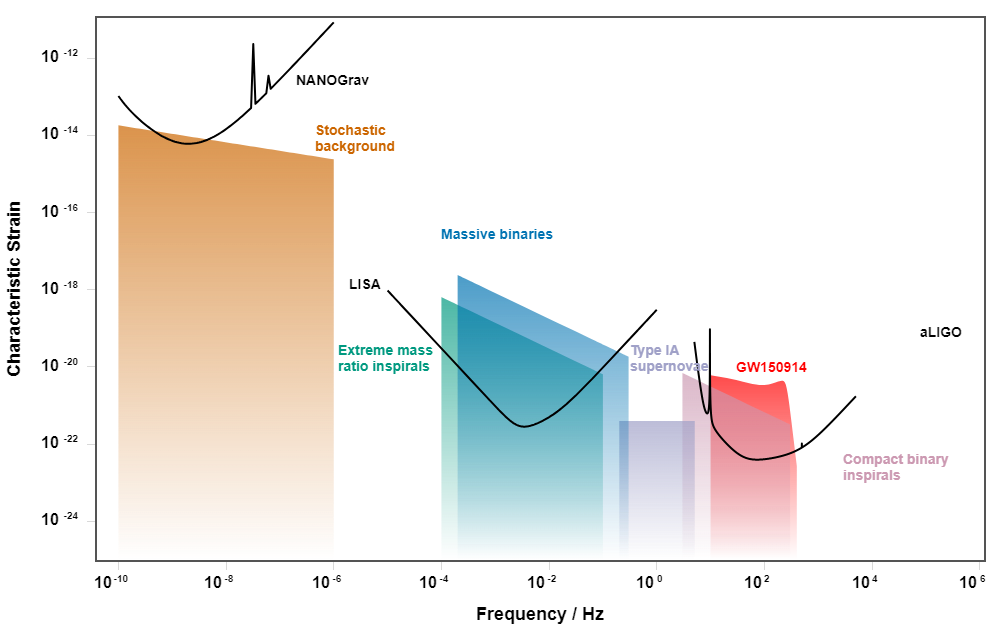
\includegraphics[width=\linewidth]{figs/my_gwplotter.png}
        \caption{My more realistic sensitivity curve approximation in GW Plotter !!
        \centering \url{https://jeremy-baier/github.io/gwplotter}
        }
        \label{fig:gwplotter_update}
    \end{figure}
\end{frame}

\begin{frame}{Conclusions}
    \begin{itemize}
        \item Sensitivity curves are a way to characterize the sensitivity of a detector to a given signal.
        \item PTA sensitivity curves are not pizza slices !!
        \item With some approximations, I derive approximate but quick sensitivity curve for PTAs.
        \item I implement quick background sensitivity curves into \textit{GW Plotter} to better represent the PTA community.
    \end{itemize}
\end{frame}

\begin{frame}{References}
    \begin{thebibliography}{1}
        \bibitem{Hazboun2019} Hazboun, J. S., Romano, J. D., Smith, T. L. (2019). Realistic sensitivity curves for pulsar timing arrays. \textit{Phys. Rev. D}, 100, 104028.
        \bibitem{Moore2015} Moore, C. J., Cole, R. H., Berry, C. P. L. (2015). Gravitational-wave sensitivity curves. \textit{Class. Quantum Grav.}, 32, 015014.
        \bibitem{Babak2024} Babak, S. et al. (2024). Forecasting PTA sensitivity. arXiv:2404.02864.
        \bibitem{Jennings2021} Jennings, R. (2021). Transmission Functions for Polynomial Fits. NANOGrav Memorandum 006.
    \end{thebibliography}
\end{frame}

\end{document}
